\section{Introdução}
O termo sistema legado descreve um sistema antigo que permanece em operação em uma organização.[1] Geralmente utilizam bancos de dados obsoletos.\footnote{https://pt.wikipedia.org/wiki/Sistema\_legado}:
\begin{enumerate}
    \item dificuldade de compreensão das regras de negócio neles implementadas;
    \item desconhecimento das razões que levaram a determinadas decisões;
    \item problemas na estruturação dos módulos de código;
    \item miscelânea de estilos de programação;
    \item obsolescência das ferramentas de desenvolvimento;
    \item impossibilidade de reaproveitamento dos equipamentos nos quais são executados para execução de softwares mais atuais;
    \item Altos custos de manutenção;
    \item Software complexo;
    \item Software de suporte obsoleto;
    \item Hardware obsoleto;
    \item Sem conhecimento técnico;
    \item Negócio crítico;
    \item Backlog de solicitações de mudança;
    \item Documentação deficiente;
    \item Conhecimento empresarial incorporado;
    \item Mal compreendido pelos mantenedores;
\end{enumerate}

Ou seja, infelizmente a Hotmart está repleta de código legado e que nascem a cada dua mais. Para se ter uma ideia, veja a quantidade de repositórios que temos hoje no GitHub:

\begin{figure}[H]
    \centering
    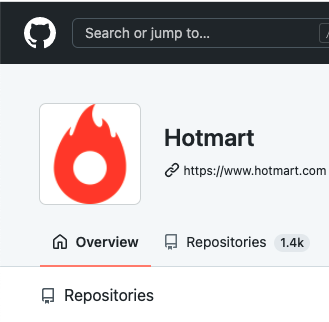
\includegraphics[scale=1,keepaspectratio=true]{images/01.png}
    \caption{Repositórios presentes no GitHub}
    \label{github_repo}
\end{figure}

Obviamente nem todos esses repositórios representam uma APP ou API, mas se formos conservadores e considerarmos 50\%, então teremos 700 repositórios onde nossas regras de negócio residem. Acho que levamos muito a sério a história de sair do monolito e acabamos criando tanto microserviço que as coisas podem ter saído um pouco do controle.

Mas então por que softwares legados existem? A resposta é simples: porque ninguém nasce sabendo aonde quer chegar. Uma empresa quando nasce, começa a ter que fazer suas escolhas. Ao longo do seu caminho, ela opta por boas ou não tão boas assim. Em um determinado momento, as escolhas passadas ajudam esta empresa a começar seguir em um caminho mais coeso. Isso se chama Maturidade.

\begin{figure}[H]
    \centering
    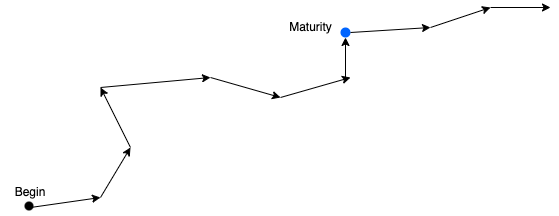
\includegraphics[scale=0.60,keepaspectratio=true]{images/02.png}
    \caption{Processo de amadurecimento}
    \label{mature_process}
\end{figure}

Se fosse possível pegarmos tudo de bom e ruim que trilhamos e juntar as melhores escolhas desde o momento em que nascemos até o momento em que amadurecemos, seria perfeito. E é exatamente o que é possível fazer com um software: a consolidação do conhecimento. 

\begin{figure}[H]
    \centering
    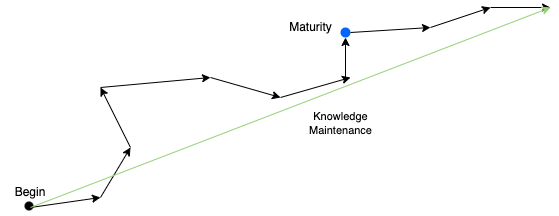
\includegraphics[scale=0.60,keepaspectratio=true]{images/03.png}
    \caption{Processo de consolidação do conhecimento}
    \label{knwledge_consolidation}
\end{figure}

Agora, mesmo que soubéssemos as melhores escolhas, de nada adiantaria chegar até aqui sem a correta manutenção de cada delas, ou seja, sendo que a cada nova decisão não fossem levadas em consideração todas as demais.

\begin{figure}[H]
    \centering
    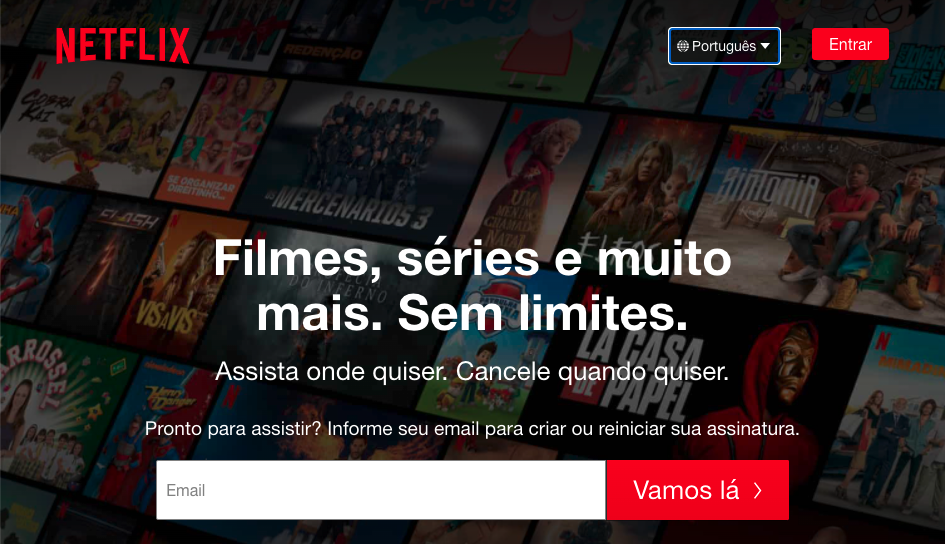
\includegraphics[scale=0.60,keepaspectratio=true]{images/04.png}
    \caption{Processo de manutenção do conhecimento}
    \label{knowledge_maintenance}
\end{figure}

Neste momento, estaríamos no que chamamos de ``Estado da Arte'' onde diversos setores da empresa poderiam trabalhar munidos de manuais para execução de seus trabalhos, deixando a parte criativa a ser utilizada no momento da criação de cada projeto. 

Em outras palavras, durante todo o processo de reconstrução do software e dos processos internos, os próprios times iriam criando sua cartilhas ou manuais de trabalho de modo que quando fosse necessário algum incremento ou atualização, todos os envolvidos já saberiam como agir tanto na demanda quanto na avaliação por pares \footnote{Pull Request, por exemplo}.

Mas se isso parece ser tão interessante, por quê nao se faz?